% ============================================================
%  TERESA: Whole-Body Active Perception for Legged
%  Robot-Assisted Emergency Assessment
%
%  IEEE Robotics and Automation Letters (RA-L) — submission draft
% ============================================================
\documentclass[journal]{IEEEtran}

% ── Packages ────────────────────────────────────────────────
\usepackage[T1]{fontenc}
\usepackage[utf8]{inputenc}
\usepackage{amsmath,amssymb,amsfonts}
\usepackage{graphicx}
\usepackage{cite}
\usepackage{url}
\usepackage{booktabs}
\usepackage{multirow}
\usepackage{xcolor}
\usepackage{hyperref}
\usepackage{bm}           % bold math symbols
\usepackage{siunitx}      % \SI{}{} units
\usepackage{acronym}      % \ac{}, \acf{}, \acp{}
\usepackage{tikz}
\usepackage{pgfplots}
\pgfplotsset{compat=1.15}
\usetikzlibrary{arrows.meta, automata, positioning, shapes.geometric,
                fit, calc, backgrounds}

% ── Macros ──────────────────────────────────────────────────
\newcommand{\R}[1]{\mathbb{R}^{#1}}
\newcommand{\vdes}{\mathbf{v}_{\mathrm{des}}}
\newcommand{\Jarm}{\mathbf{J}_{\mathrm{arm}}}

% ── Title / Authors ─────────────────────────────────────────
\title{TERESA: Whole-Body Active Perception for Legged
       Robot-Assisted Emergency Assessment}

\author{Andrea~D'Antona,~\IEEEmembership{}
        
                \thanks{A.~D'Antona is with the Department of Engineering,
                University of Ferrara, 44122 Ferrara, Italy
                (e-mail: dntndr1@unife.it).}}

% ============================================================
\begin{document}

\maketitle

% ── Acronym definitions ─────────────────────────────────────
% ============================================================
%  ACRONYMS — definitions only, not printed in PDF
%  \acrodef does not generate any output.
%  Usage in text:
%    \ac{FAST}   → first use: "Focused Assessment ... (FAST)", then: "FAST"
%    \acf{FAST}  → always full form
%    \acp{DOF}   → plural (DOFs)
%    \Ac{WBC}    → capitalised first word
% ============================================================
\acrodef{ABCDE}{Airway, Breathing, Circulation, Disability, Exposure}
\acrodef{TERESA}{Trustworthy Emergency Robot for Efficient Scanning and Assistance}
\acrodef{FAST}{Focused Assessment with Sonography in Trauma}
\acrodef{WBC}{Whole-Body Control}
\acrodef{QP}{Quadratic Program}
\acrodef{FSM}{Finite State Machine}
\acrodef{DOF}{Degree of Freedom}
\acrodef{EE}{End-Effector}
\acrodef{IK}{Inverse Kinematics}
\acrodef{FK}{Forward Kinematics}
\acrodef{MPC}{Model Predictive Control}
\acrodef{YOLO}{You Only Look Once}
\acrodef{ROS}{Robot Operating System}
\acrodef{DDS}{Data Distribution Service}
\acrodef{RGBD}{RGB-D}
\acrodef{KF}{Kalman Filter}
\acrodef{JTC}{Joint Trajectory Controller}
\acrodef{PID}{Proportional-Integral-Derivative}
\acrodef{PD}{Proportional-Derivative}
\acrodef{RNEA}{Recursive Newton-Euler Algorithm}
\acrodef{COCO}{Common Objects in Context}
\acrodef{TF}{Transform}
\acrodef{GPU}{Graphics Processing Unit}
\acrodef{NLF}{Neural Localizer Fields}
\acrodef{SMPL}{Skinned Multi-Person Linear}
\acrodef{COCO}{Common Objects in Context}


% ── Abstract ────────────────────────────────────────────────
% ============================================================
%  ABSTRACT
% ============================================================
\begin{abstract}

\draft{Deploying legged mobile manipulators for autonomous emergency
assessment requires the robot to actively adapt its body posture to the
perceptual demands of each mission phase---locating, approaching, scanning,
and performing ultrasound on an unknown patient.}

This paper presents \ac{TERESA}, an autonomous emergency assessment system on the
Boston Dynamics Spot quadruped with a Unitree Z1 arm (\draft{hereafter Spotzi}). \draft{\ac{TERESA} treats body posture as an active perceptual
resource, adapting it to the demands of four sequential phases:
(1) the robot searches for the patient by walking forward while
sweeping body posture; (2) it approaches while concurrently scanning
the torso, eliminating idle time; (3) it executes an exposure scan
covering the body surface and detecting injuries; and (4) it performs
\ac{FAST} ultrasound with pre-planned posture optimisation for each
anatomical target. A web-based interface allows the \draft{remote} operator to click
any scanned body point and trigger a full-body reconfiguration to
revisit it.}

\draft{Experiments on the Spotzi platform in a laboratory
environment, with a medical training manikin, demonstrate fully autonomous
execution of all four phases.}
\end{abstract}


% ── Keywords ────────────────────────────────────────────────
\begin{IEEEkeywords}
Whole-body active perception, legged manipulation, medical robotics,
emergency assessment, mobile manipulation, body reconfiguration.
\end{IEEEkeywords}

% ── Sections ────────────────────────────────────────────────
% ============================================================
%  I. INTRODUCTION
% ============================================================
\section{Introduction}
\label{sec:introduction}

\IEEEPARstart{E}{mergency} assessment protocols---including the \ac{ABCDE}
survey~\cite{thim2012abcde} and Focused Assessment with Sonography in Trauma (\ac{FAST})
ultrasound~\cite{rozycki1996}---enable rapid triage of life-threatening
conditions at the point of care. In mass-casualty
incidents and disaster sites, however, trained personnel are often unavailable,
creating a critical bottleneck.

Legged platforms such as the Boston Dynamics Spot can traverse stairs, rubble,
and confined spaces inaccessible to wheeled robots, and can therefore reach
patients wherever they lie. Navigation alone, however, is insufficient:
emergency assessment requires physical interaction with the patient---checking
airway patency and respiratory effort, inspecting the skin for signs of poor
circulation, scanning the body surface for wounds, burns, and haemorrhages, and
performing ultrasound at specific anatomical targets. A manipulator arm extends the robot's reachable
workspace, enables multiple viewpoints of the same body region, and provides the
dexterity needed for compliant probe contact.

% ── Related Work ─────────────────────────────────────────────

Robot-assisted ultrasound has advanced over two decades on fixed-base
platforms. Comprehensive surveys~\cite{vonhaxthausen2021,li2021overview}
document the evolution from teleoperated systems to autonomous scanning, and
Hidalgo et al.~\cite{hidalgo2023} review current clinical applications. Key
technical advances include active-sensing end-effectors~\cite{ma2022} and
autonomous protocol execution~\cite{suligoj2021,farsoni2025autonomous}. 

\draft{The Exposure phase of \ac{ABCDE} requires systematic visual
inspection of the body surface for wounds, burns, and haemorrhages.
Open-vocabulary detectors such as Grounding
DINO~\cite{liu2023groundingdino} enable zero-shot injury detection without
task-specific training data. Combined with depth back-projection from the
RGB-D stream, these models produce metric 3D injury locations.}
\draft{To plan the exposure scan grid and the \ac{FAST} the robot must first estimate
the patient's 3D body pose.} Neural Localizer Fields
(NLF)~\cite{isarandi2024nlf} \draft{regress 24-joint \ac{SMPL}
skeletons from monocular RGB, providing full anatomical coverage beyond the
standard 17-keypoint \ac{COCO} format.}
%Addressing uncertainty in human-centered robotics,
%Casado et al.~\cite{casado2025navigating} proposed diffusion-based intention
%estimation for shared wheelchair control---a theme that similarly motivates
%\ac{TERESA}'s quality-driven perception loop.
Despite
this progress, all deployed systems share a fundamental limitation: the patient
must be pre-positioned within the arm's reachable workspace, confining
autonomous ultrasound and scanning to controlled clinical settings. A possible solution is achieved by the 
modern \ac{WBC}. This builds on operational space formulation~\cite{khatib1987},
manipulability analysis~\cite{yoshikawa1985}, and optimisation-based
control~\cite{wensing2023}. These principles have been extended to legged
manipulators through hierarchical \ac{MPC}~\cite{sleiman2021},
\ac{QP}-based formulations~\cite{li2022wbc}, holistic~\cite{haviland2022} and
Spot-specific grasping and manipulability enhancement~\cite{zimmermann2021,xie2024manip}.
Across this body of work, however, the manipulation target is assumed known or
static; no formulation accounts for the coupling between body posture and the
quality of perceptual data used to localise that target in the first place.


Active perception research has established that deliberate sensor motion
systematically outperforms passive observation~\cite{zeng2020,bai2021,zaky2020}.
This insight has been operationalised through perception-aware
planning~\cite{zhang2020fisher,tordesillas2022}, next-best-view
grasping~\cite{breyer2022}, view planning for pose estimation~\cite{hu2022}, and
active neural sensing~\cite{ren2023}. When applied to mobile manipulation,
whole-body interaction~\cite{mittal2022}, coupled
perception-manipulation~\cite{xie2024capm} and one-shot multimodal
frameworks~\cite{qin2026} have demonstrated trajectory optimisation for
information gain. Critically, all of these systems operate on wheeled bases
whose body posture is fixed: the base provides mobility but does not participate
in shaping the perceptual field. Conversely, work on posture optimisation for
legged systems---through reachability
analysis~\cite{makhal2018,zhao2025}, base placement~\cite{fan2021},
body-ground contact~\cite{wolfslag2020}, and the broader legged manipulation
literature~\cite{gong2023}---treats perception as a static input to the motion
planner rather than as a quantity to be optimised. No existing system closes the
perception-action loop at the whole-body level on a legged platform for medical
tasks.

% ── Gap & Challenge ──────────────────────────────────────────

We advocate a paradigm in which body posture on a legged
platform is treated as a first-class perceptual resource: the robot actively
adapts its height, pitch, and yaw to maximise the quality of its own
perceptual input, rather than solely to minimise kinematic error. The key
idea is to close the perception-action loop at the whole-body level through
confidence-gated search and anticipatory scanning.

% ── TERESA ───────────────────────────────────────────────────

This paper presents \acf{TERESA} (Fig.~\ref{fig:system_overview}), an integrated
system for autonomous emergency assessment on the Boston Dynamics Spot legged
robot equipped with a Unitree Z1 manipulator arm --- \draft{Spotzi}.
Building on the fixed-base ultrasound scanning competence
established in~\cite{farsoni2025autonomous}, \ac{TERESA} extends autonomous
assessment to a fully mobile platform. \draft{We target the Exposure
and \ac{FAST} phases of \ac{ABCDE} because they share the same hardware
configuration and impose nearly identical whole-body coordination
demands.} \ac{TERESA} addresses this through a unified whole-body active
perception framework that treats body posture as an explicit control resource
across all four phases.

% ── Contributions ────────────────────────────────────────────

The key contributions of this paper are as follows.
\begin{enumerate}
  \item \textbf{Whole-body active perception framework} in which body
        posture is optimised to improve perceptual quality rather than
        solely to minimise kinematic error
        (Section~\ref{sec:active_perception}).
  \item \textbf{Confidence-gated search with dual-sensor locking} that
        combines forward base search with body pitch sweep, ensuring robust
        patient localisation before committing to navigation.
  \item \textbf{Exposure body scanning pipeline} integrating an adaptive
        skeleton-keypoint grid with zero-shot Grounding DINO injury
        detection and an interactive web-based review interface
        (Sections~\ref{sec:active_perception}
        and~\ref{sec:system_architecture}).
  \item \textbf{Pre-planned body reconfiguration} that searches over body
        height, pitch, and base displacement to place each anatomical target
        in the arm's preferred manipulation region
        (Section~\ref{sec:body_reconf}).
  \item \textbf{Experimental validation} on the \draft{Spotzi}
        platform demonstrating fully autonomous execution of all four phases
        (Section~\ref{sec:experimental_results}).
\end{enumerate}

To the best of our knowledge, \ac{TERESA} is the first legged robotic system to
demonstrate perception-driven whole-body reconfiguration for autonomous
emergency assessment.

% ── Outline ──────────────────────────────────────────────────

\draft{The remainder is organised as follows:
Section~\ref{sec:problem_formulation} formulates the problem,
Section~\ref{sec:active_perception} presents the whole-body active perception
framework, Section~\ref{sec:system_architecture} details the system
architecture and mission \ac{FSM},
Section~\ref{sec:experimental_results} reports experimental results, and
Section~\ref{sec:conclusion} concludes.}

% ============================================================
%  II. PROBLEM STATEMENT
% ============================================================
\section{Problem Statement}
\label{sec:problem_formulation}

\subsection{System Model}

The \ac{TERESA} platform consists of a Boston Dynamics Spot quadruped and a
Unitree Z1 six-\ac{DOF} arm rigidly mounted on the robot's back. Four frames
are defined: the world frame $\mathcal{F}_W$ (coincident with Spot odometry),
the body frame $\mathcal{F}_B$, the arm base frame $\mathcal{F}_0$ (fixed
relative to $\mathcal{F}_B$), and the end-effector frame $\mathcal{F}_{EE}$ (at
the Z1 flange). The Spot base is modelled as a non-holonomic vehicle with
configuration $\boldsymbol{\xi} = [x,\, y,\, \theta]^\top \in \mathbb{R}^2
\times \mathbb{S}^1$, constrained to forward velocity $v_x$ and yaw rate
$\omega_z$:
\begin{equation}
\dot{\boldsymbol{\xi}} =
\begin{bmatrix} \cos\theta \\ \sin\theta \\ 0 \end{bmatrix} v_x
+
\begin{bmatrix} 0 \\ 0 \\ 1 \end{bmatrix} \omega_z.
\label{eq:nonholonomic}
\end{equation}

The body posture is parametrised by height $h$ and pitch $\varphi$, commanded
through the native posture control interface, with bounds
$h \in [h_{\min},\, h_{\max}]$, $\varphi \in [0,\, \varphi_{\max}]$. The Z1 arm
has $n = 6$ revolute joints $\mathbf{q} \in \mathbb{R}^6$ with geometric
Jacobian $\mathbf{J}_{\mathrm{arm}}(\mathbf{q}) \in \mathbb{R}^{6 \times 6}$.
The combined control input during the approach phase is
$\mathbf{u} = [\dot{\mathbf{q}},\, v_x,\, \omega_z]^\top \in \mathbb{R}^8$.

\subsection{Task Definition}

An autonomous emergency assessment mission requires the \ac{EE} to reach a
sequence of $N$ anatomical target poses
$\mathcal{T} = \{\mathbf{T}_i^* \in SE(3)\}_{i=1}^{N}$ (e.g., \ac{FAST}
quadrants). The targets are not known a priori---they are estimated during the
mission from the onboard \ac{RGBD} cameras, which are the only source of
perception.

\subsection{Problem}

Given the system model and the unknown patient position, find control inputs
$\mathbf{u}(t)$ and body posture commands $(h(t), \varphi(t))$ that enable the
robot to: (i)~discover a posture from which detection confidence exceeds a
threshold, ensuring robust patient localisation before committing to the
approach; (ii)~navigate to a configuration from which all targets in
$\mathcal{T}$ are reachable; (iii)~reconfigure its body to maximise arm
manipulability for each scanning target; and (iv)~bring the \ac{EE} to each
target pose with bounded error $\|\mathbf{p}_{EE} - \mathbf{p}_i^*\| \leq
\varepsilon_p$.

\subsection{Assumptions}

The following assumptions are adopted: the patient remains stationary during
scanning (A1); Spot operates on flat terrain (A2); the rigid transform between
$\mathcal{F}_B$ and $\mathcal{F}_0$ is known and constant (A3); a single
patient is present (A4); and no external perception infrastructure is available
(A5).

% ============================================================
%  III. WHOLE-BODY ACTIVE PERCEPTION AND CONTROL
% ============================================================
\section{Whole-Body Active Perception and Control}
\label{sec:active_perception}

The core contribution of \ac{TERESA} is a whole-body active perception
framework: the robot continuously adapts its posture---body height, pitch, and
yaw---to maximise perceptual quality. This section describes how each of the
four mission phases defined in Section~\ref{sec:problem_formulation} is
resolved: hybrid confidence-gated search (Phase~A), anticipatory approaching
with concurrent scanning (Phase~B), exposure body inspection with interactive
review (Phase~C), and \ac{FAST} ultrasound acquisition with compliant contact
(Phase~D).

The term \emph{whole-body} here denotes a perceptual extension of the classical
\ac{WBC} principle. Whereas traditional \ac{WBC} coordinates all degrees of
freedom to minimise kinematic error, \ac{TERESA} extends this coordination to
the perceptual domain: body posture---height, pitch, and yaw---is treated as an
explicit control resource that shapes the robot's sensory field. By commanding
posture to improve what the robot sees, at higher resolution and from more
informative viewpoints, \ac{TERESA} elevates the legged base from a passive
transport platform to an active participant in the perception-action loop. This
principle underpins every phase of the mission, from searching through
approaching to scanning.

\subsection{Phase A --- Searching}
\label{sec:phase_searching}

Before the robot can approach the patient, it must first localise them
reliably. In an unstructured emergency scenario, the patient's position is
unknown a priori. The \ac{EE}-mounted RealSense benefits from the Z1 arm's full
six-\ac{DOF} mobility, which can orient the camera in any direction without
moving the base. The body-mounted Orbbec, however, has a fixed orientation
relative to Spot: its downward field of view depends entirely on body pitch,
making pitch the only posture parameter that directly improves its detection of
a patient lying on the ground. \ac{TERESA} therefore avoids time-consuming base
rotations and instead searches by walking forward while sweeping body pitch.

\subsubsection{Forward search with pitch sweep}

The robot walks forward at low speed while the body pitch is adjusted through
a sequence of angles $\varphi \in [0, \varphi_{\max}]$. At each pitch, two
cameras observe the environment in complementary roles. The body-mounted Orbbec
runs YOLO11-pose and a posture classifier that outputs a confidence score
$c \in [0, 1]$. The \ac{EE}-mounted RealSense, actively oriented by the Z1
arm, runs a torso tracker that scans the surroundings independently of the
base heading. Two conditions are evaluated:

\begin{itemize}
  \item \textbf{Orbbec direct detection}: if the body-mounted camera detects a
        lying patient with high confidence at the current pitch, the robot
        transitions immediately to target locking.
  \item \textbf{RealSense guidance}: if the \ac{EE} camera detects a potential
        body while the Orbbec has not yet confirmed, the robot enters a
        semi-locking phase. It walks toward the detected torso and adjusts
        pitch to give the Orbbec a clean observation window.
\end{itemize}

If neither condition is met after the pitch sweep, the robot continues walking
forward and repeats the sweep, progressively covering the search area without
the idle time of discrete base rotations. This strategy exploits the arm's
native mobility for rotational search while using body pitch---the one viewing
parameter the arm cannot compensate for---to optimise the Orbbec's fixed
viewpoint.

\subsubsection{Dual-sensor confidence lock}

Patient localisation is confirmed through a hybrid lock that fuses information
from both cameras. When the Orbbec detects a lying posture with high
confidence, the robot enters a locking state: the arm returns to an elevated
home pose, and the coordinator collects a sequence of approach point estimates
in the world-fixed odometry frame $\mathcal{F}_W$, computing their mean as the
navigation target. Concurrently, the NLF pipeline produces a refined 3D
skeleton estimate by accumulating two valid detections with exponential moving
average smoothing, providing higher-fidelity anatomical data for the subsequent
approach phase. The transition to the approach phase is gated by both the
arm's home trajectory and the collection of the required number of samples. If
the Orbbec detection is temporarily lost, the system tolerates a brief absence
before resuming the search from the current position.

\subsection{Phase B --- Approaching}
\label{sec:phase_approaching}

In traditional mobile manipulation pipelines, the robot first navigates to a
target position, stops, and only then begins visual scanning---a sequential
approach that introduces significant idle time. \ac{TERESA} eliminates this
idle period by executing the body scan concurrently with the approach
navigation.

\subsubsection{Whole-body coordination}

During the approach, two independent controllers run in parallel. The Spot base
is driven by a proportional controller that computes $v_x$ and $\omega_z$ from
the distance and angle to the target in $\mathcal{F}_W$. The arm is controlled
by a \ac{WBC} formulation that orients the \ac{EE}-mounted RealSense toward the
patient's torso centroid. The joint velocities are computed via a damped
pseudo-inverse of the arm Jacobian:
\begin{equation}
\dot{\mathbf{q}} = \mathbf{J}_{\mathrm{arm}}^\top
\bigl(\mathbf{J}_{\mathrm{arm}} \mathbf{J}_{\mathrm{arm}}^\top
+ \mu\,\mathbf{I}_6\bigr)^{-1} \mathbf{v}_{\mathrm{des}},
\label{eq:damped_pinv}
\end{equation}
where $\mu > 0$ is a damping factor that prevents singularities near
kinematic limits, and $\mathbf{v}_{\mathrm{des}} \in \mathbb{R}^6$ is the
desired end-effector spatial velocity. The damped pseudo-inverse solves
$\mathbf{J}_{\mathrm{arm}} \dot{\mathbf{q}} = \mathbf{v}_{\mathrm{des}}$ in a
least-squares sense, mapping a commanded \ac{EE} motion to the joint space.
Here only the angular component of $\mathbf{v}_{\mathrm{des}}$ is active: it
encodes the rotation required to align the RealSense camera with the look-at
direction $\mathbf{x}_{EE} = (\mathbf{p}^* -
\mathbf{p}_{EE})/\|\mathbf{p}^* - \mathbf{p}_{EE}\|$, keeping the patient's
torso centred in the frame. The translational component of
$\mathbf{v}_{\mathrm{des}}$ is zero, as the arm holds a nominal home position
during approach. The base velocity is modulated by a
QualityMonitor that scales the approach speed in proportion to detection
confidence, avoiding premature commitment to uncertain targets while preventing
unnecessary stops.

\subsubsection{Adaptive anticipatory scan grid}

The arm executes a perceptual body scan using a dynamically generated Cartesian
grid of poses around the current \ac{EE} position. During the pre-approach
phase, the RealSense tracker publishes per-keypoint confidence scores for the
four torso landmarks (shoulders and hips), which drive the grid generation. If
all four keypoints are detected with high confidence, the scan uses a minimal
two-pose grid: the current \ac{EE} pose advanced toward the patient plus an
elevated viewpoint. If any keypoint falls below the threshold, the grid expands
to a three-pose comprehensive pattern with symmetric lateral offsets, an
elevated frontal viewpoint, and the home pose interleaved between lateral
transits. All scanning poses include a forward advance toward the patient. At
each pose, depth and skeleton data are fused into 3D keypoint estimates via a
weighted average accounting for detection rate and spatial stability. From the
fused torso model, the five canonical \ac{FAST} target poses are computed as
fixed offsets from the estimated torso centroid in $\mathcal{F}_0$.

\subsection{Phase C --- Exposure}
\label{sec:phase_exposure}

After the anticipatory scanner has localised the patient's anatomy, Phase~C
executes a systematic visual inspection of the body surface, serving the ``E''
(Exposure) component of the \ac{ABCDE} protocol. A key design principle is that
the operator remains in the loop: the system automates the scanning motion but
preserves the clinician's ability to inspect, re-examine, and override.

\subsubsection{Posture optimisation for body reconfiguration}
\label{sec:body_reconf}

Once the anticipatory body scanner has localised the patient's anatomy and
computed the target set $\mathcal{T}$ (both \ac{FAST} ultrasound targets and
exposure grid points) in $\mathcal{F}_W$, the system pre-plans an optimal body
posture for each target through a two-tier kinematically-aware stance search
with \ac{IK}-driven retry. This optimisation is shared with Phase~D
(Section~\ref{sec:phase_fast}).

The posture optimisation space spans three parameters: body height $h \in
[h_{\min}, h_{\max}]$ and pitch $\varphi \in [0, \varphi_{\max}]$, as defined
in Section~\ref{sec:problem_formulation}, plus a body-frame base displacement
$dy \in \mathbb{R}$ along the patient's head-to-foot axis, expressed in the
patient-aligned body frame (Section~\ref{sec:system_architecture}).
The discrete search grids are $\mathcal{H} = \{h_1, \dots, h_{N_h}\}$ and
$\mathcal{P} = \{\varphi_1, \dots, \varphi_{N_p}\}$, with $dy$ sampled
uniformly at \SI{0.10}{\metre} intervals.  The cost function includes a
regularisation term that penalises lateral displacement:
\begin{equation}
  J(h, \varphi, dy) =
  \bigl\|\mathbf{T}_{\mathcal{F}_W}^{\mathcal{F}_0}(h, \varphi, dy)\,
  \mathbf{p}^* - \mathbf{p}_{\mathrm{sweet}}\bigr\|
  + \lambda\,|dy|,
  \label{eq:posture_cost}
\end{equation}
where $\mathbf{p}_{\mathrm{sweet}} \in \mathbb{R}^3$ is the empirically
determined centre of the Z1 arm's preferred manipulation region in
$\mathcal{F}_0$, and $\lambda = 0.50$ weights lateral movement against
reachability.  The value $\lambda=0.50$ was chosen empirically to balance
reachability against energy cost: $\lambda>1.0$ prevented necessary base
displacement, while $\lambda<0.25$ caused excessive walking for marginal
reachability gains.  This penalty encourages the optimiser to prefer height and pitch
adjustments over base walking---reducing energy consumption and producing
smoother, more predictable motion---while still allowing longitudinal
displacement when strictly necessary.  The two-tier escalation proceeds as
follows:

\begin{enumerate}
  \item \textbf{2D search}---$(h, \varphi)$ only: a coarse grid sweeps
        $\mathcal{H} \times \mathcal{P}$ ($N_h N_p$ combinations, typically
        12).  For each candidate, the system transforms the target to
        $\mathcal{F}_0$ and queries the \ac{IK} solver.  If a posture yields
        a solution within a \SI{2}{\second} timeout, it is selected.
  \item \textbf{3D escalation}---$(dy, h, \varphi)$: when the 2D search fails,
        the optimiser adds longitudinal base displacement $dy$ (Spot walks
        along the patient's body), expanding to $N_{dy} N_h N_p$
        combinations.  If the \ac{IK} solver also times out at this tier, the
        point is skipped---the arm cannot reach it even with full base
        repositioning.
\end{enumerate}

The optimisation is computed once per target after $\mathcal{T}$ is available,
imposing no real-time computational burden.  Body reconfiguration is executed
between targets: Spot assumes the pre-computed posture $(h_i^*, \varphi_i^*)$,
settles, and the base navigator drives the $dy$ displacement before the Z1 arm
executes the \ac{IK} trajectory toward the transformed target.

\subsubsection{Posture-adaptive scan grid}

The scan grid adapts to the patient's estimated body pose. Four torso
keypoints---left and right shoulders, left and right hips---define a bilinear
patch over the body surface.  Let $\mathbf{p}_{SL}, \mathbf{p}_{SR},
\mathbf{p}_{HL}, \mathbf{p}_{HR} \in \mathbb{R}^3$ denote these keypoints in
$\mathcal{F}_W$.  The grid is generated by interpolating uniformly along the
two parametric directions: head-to-foot ($u$-axis, from shoulders to hips) and
lateral ($v$-axis, from left to right).  A grid point at parameters
$(u, v) \in [0,1] \times [0,1]$ is computed as
$\mathbf{p}(u,v) = (1{-}u)(1{-}v)\,\mathbf{p}_{SL} + u(1{-}v)\,\mathbf{p}_{HL}
+ (1{-}u)v\,\mathbf{p}_{SR} + uv\,\mathbf{p}_{HR}$, with a fixed height offset
to maintain a safe camera-to-skin distance.  Typical grid resolution is
\SI{0.15}{\metre} in both directions, producing 15--25 points depending on
torso dimensions.  When the NLF prior is available, all 24 \ac{SMPL} joints
are populated, extending the grid to the head, hands, and feet for full-body
coverage.  Grid points are visited in a serpentine path to minimise arm
travel.

\subsubsection{Injury detection}

At each grid point, Grounding DINO---a zero-shot
open-vocabulary object detector---runs on the RealSense RGB stream at
approximately 1\,fps on the Jetson Orin GPU, prompted with a vocabulary
of wound-related terms (wound, laceration, bleeding, burn, etc.). Detections
are projected to 3D world coordinates via the registered depth channel and
associated with their grid point index.

\subsubsection{Web-based interactive review}

Following the sweep, the system enters an interactive review phase: the web
interface overlays the exposure grid on the RealSense feed with detected
injuries highlighted as colour-coded bounding boxes.  The operator can click
any grid point to command the robot to return to that body region for
re-inspection.  The full re-positioning mechanism---posture optimisation,
settle, base navigation, and \ac{IK} trajectory replay---is detailed in
Section~\ref{sec:system_architecture}.  A termination command ends the review
and advances the mission to Phase~D.

\subsection{Phase D --- \acs{FAST}}
\label{sec:phase_fast}

Phase~D performs autonomous ultrasound acquisition at the $N$ \ac{FAST}
targets estimated during Phase~B. Body posture optimisation for each
$\mathbf{T}_i^* \in \mathcal{T}$ follows the same two-tier procedure described
in Section~\ref{sec:body_reconf}, applied to the \ac{FAST} target set. The
distinctive requirement of this phase is compliant probe contact with the
patient's body surface.

\subsubsection{Contact control}

The Unitree Z1 does not provide native impedance control, yet ultrasound
scanning requires compliant probe contact. \ac{TERESA} implements a custom
Cartesian impedance controller on the Z1 torque interface at \SI{500}{\hertz}.
The desired \ac{EE} pose is computed relative to the torso surface centroid
$\mathbf{p}_s$ and outward normal $\mathbf{n}_s$, placing the probe at
$\mathbf{p}_{\mathrm{des}} = \mathbf{p}_s + d\,\mathbf{n}_s$, where $d$ is the
desired contact offset.  Joint torques are computed as
\begin{equation}
\boldsymbol{\tau} = \mathbf{J}_{\mathrm{arm}}(\mathbf{q})^\top
\bigl[\mathbf{K}_p(\mathbf{p}_{\mathrm{des}} - \mathbf{p}_{EE})
- \mathbf{K}_d\,\dot{\mathbf{p}}_{EE}\bigr]
+ \mathbf{g}(\mathbf{q}) + \mathbf{C}(\mathbf{q}, \dot{\mathbf{q}}),
\label{eq:impedance}
\end{equation}
where $\mathbf{K}_p, \mathbf{K}_d \in \mathbb{R}^{3 \times 3}$ are adaptive
stiffness and damping gains that scale linearly with arm extension to prevent
overloading at the workspace boundary, $\mathbf{g}(\mathbf{q})$ and
$\mathbf{C}(\mathbf{q}, \dot{\mathbf{q}})$ are the gravity and Coriolis terms
computed via Pinocchio~\cite{carpentier2019pinocchio}, and
$\dot{\mathbf{p}}_{EE} = \mathbf{J}_{\mathrm{arm}}(\mathbf{q})\,
\dot{\mathbf{q}}$ is the end-effector velocity.  A safe switching service
alternates between the impedance controller and a position-controlled joint
trajectory controller, defaulting to position control on error.

% ============================================================
%  IV. SYSTEM ARCHITECTURE
% ============================================================
\section{System Architecture}
\label{sec:system_architecture}

The \ac{TERESA} system is organised into four layers---hardware, perception,
mission management, and control---communicating over \ac{ROS}~2 with
\ac{DDS}.

\subsection{Hardware Platform}

The hardware platform, shown in Fig.~\ref{fig:system_overview}, carries two
\ac{RGBD} cameras with complementary roles. An Orbbec Femto Bolt is body-mounted
for wide-field patient detection at distances up to \SI{3}{\metre}. An Intel
RealSense D435 is mounted at the Z1 \ac{EE} and positioned by the arm's look-at
controller as an active pan-tilt unit for close-range torso tracking and surface
estimation. Spot's five built-in stereo cameras are positioned low on the body
for ground-plane obstacle avoidance and are not suitable for skeleton detection.
Computation is distributed across two units: Spot's onboard computer SpotCore
handles base control and odometry, while an NVIDIA Jetson Orin AGX runs
perception, arm control, mission coordination, and \ac{WBC} via Docker
containers with CUDA 11.4.

%\subsection{Frame Tree}
%
%The \ac{TF} tree defines the spatial relationships between all system
%components, as illustrated in Fig.~\ref{fig:frame_tree}. The root
%\texttt{my\_spot/odom} is world-fixed and published by SpotCore odometry.
%\texttt{my\_spot/body} moves with the base (height, pitch, and yaw are set
%via \texttt{/body\_pose}) and branches into the Orbbec chain
%(\texttt{orbbec\_link} $\to$ \texttt{orbbec\_color\_optical\_frame}) and the Z1
%arm chain (\texttt{world} $\to$ \texttt{link00} $\to$ $\cdots$ $\to$
%\texttt{link06} $\to$ \texttt{camera\_link} $\to$
%\texttt{camera\_color\_optical\_frame}). Because the \texttt{body $\to$ world}
%transform is static, any change in body posture automatically propagates to the
%arm base frame $\mathcal{F}_0$.

%\begin{figure}[t]
%  \centering
%  % ============================================================
%  FRAME TREE — TF hierarchy with hardware-based coloring
%  Requires: tikz
% ============================================================
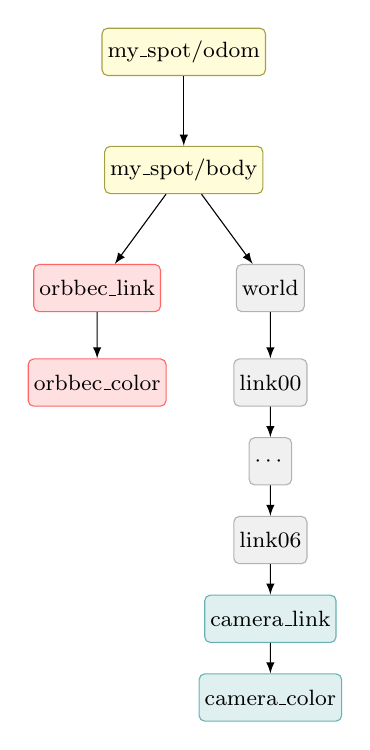
\begin{tikzpicture}[
    level 1/.style={sibling distance=40mm},
    level 2/.style={sibling distance=22mm},
    level 3/.style={level distance=12mm},
    level 4/.style={level distance=10mm},
    every node/.style={draw, rounded corners=2pt, font=\footnotesize,
                       inner sep=2pt, minimum height=6mm},
    edge from parent/.style={draw, -latex},
    spot/.style  = {fill=yellow!15,  draw=yellow!60!black},
    z1/.style    = {fill=gray!12,   draw=gray!60},
    orbbec/.style = {fill=red!12,   draw=red!60},
    rs/.style    = {fill=teal!12,   draw=teal!60},
  ]
  \node[spot] {my\_spot/odom}
    child { node[spot] {my\_spot/body}
      child { node[orbbec] {orbbec\_link}
        child { node[orbbec] {orbbec\_color} }
      }
      child { node[z1] {world}
        child { node[z1] {link00}
          child { node[z1] {$\cdots$}
            child { node[z1] {link06}
              child { node[rs] {camera\_link}
                child { node[rs] {camera\_color} }
              }
            }
          }
        }
      }
    };
\end{tikzpicture}

%  \caption{\ac{TF} frame tree. \texttt{my\_spot/odom} $\to$
%           \texttt{my\_spot/body} branches into the Orbbec chain and the Z1 arm
%           chain.}
%  \label{fig:frame_tree}
%\end{figure}

\subsection{Mission Management and System Integration}

The mission is orchestrated by a 13-state \ac{FSM}
(Fig.~\ref{fig:fsm}), organised into the four phases of
Section~\ref{sec:problem_formulation}. After Waiting TF and Idle ensure system
readiness, the \ac{FSM} enters Phase~A (Searching). The robot first walks the base
forward while adjusting body pitch to bring the patient into the cameras' field
of view---this is the SEARCHING state. When the RealSense detects a potential
torso, the system uses that coarse guidance to walk toward the detection and
adjust pitch, giving the Orbbec a clean observation window; we call this
SEMI\_LOCKING. If the Orbbec then confirms a lying patient with high
confidence, the system advances to LOCKING, where the NLF pipeline produces a
refined 3D skeleton and the coordinator collects approach point estimates.
Timeouts at any point revert to SEARCHING, ensuring the robot does not commit
to a false detection.

Phase~B (Approaching) begins once a stable lock is achieved. The robot first
drives toward the target while the anticipatory body scanner builds the torso
model---a state we call PRE\_APPROACH---then transitions to APPROACHING, where
the \ac{WBC} \ac{QP} coordinates base velocity and arm look-at control
concurrently, keeping the camera on the patient throughout the approach.

Phase~C (Exposure) starts after the approach handoff. An optional Waiting
Exposure gate lets the operator confirm before the scan begins. The system then
enters EXPOSURE\_SCANNING, executing a multi-view body surface inspection with
Grounding DINO injury detection at each grid point. Once the sweep is complete,
the \ac{FSM} moves to EXPOSURE\_REVIEW: the operator can click any grid point
in the web interface to trigger a full re-positioning and re-inspection,
remaining in this state until explicitly terminated.

Phase~D (\acs{FAST}) follows, with an analogous Waiting FAST gate for manual
confirmation. The SCANNING state executes ultrasound acquisition under
pre-planned body reconfiguration, one target at a time. When a target is
kinematically unreachable from the current posture, the system temporarily
enters WS\_EXTENSION, walking the base along the patient's body to extend the
workspace, then loops back to SCANNING with the new \ac{IK} solution.

Transitions are triggered by perception confidence (dashed edges in
Fig.~\ref{fig:fsm}) or geometric conditions (solid edges); the mission
completes by returning to Idle.

Fig.~\ref{fig:system_block} shows the complete system architecture in six
layers.  The Orbbec and RealSense \ac{RGBD} streams feed the Perception layer,
which runs YOLO-pose skeleton detection, Kalman-filtered 3D back-projection,
NLF 3D body pose estimation, surface estimation, and Grounding DINO injury
detection.  Perception outputs route to the 13-state Mission \ac{FSM}, which
enables four Planning modules: the Exposure Scanner, the \ac{FAST} Ultrasound
planner, the Body Pose Optimizer, and the Web UI for interactive review.  The
Control layer translates plans into actuation: the \ac{WBC} \ac{QP} publishes
base velocity $[v_x,\,\omega_z]$ to Spot and arm goals to the \ac{IK} Goal
Multiplexer; the Impedance Controller manages compliant contact during
\ac{FAST} scanning, publishing joint torques $\boldsymbol{\tau}$ directly to
the Z1.  The Z1 \ac{FSM} manages the arm's internal state
transitions---homing, look-at tracking, scanning trajectory execution, and
impedance-controlled contact---and synchronises with the \ac{WBC} coordinator.
Dashed arrows in the diagram denote operator-triggered or posture-optimisation
paths.  An emergency stop immediately halts the base and returns the arm to a
safe configuration.

\begin{figure*}[t]
  \centering
  \resizebox{\textwidth}{!}{% ============================================================
%  FSM DIAGRAM — 13 states, 4 columns
%  Requires: tikz
% ============================================================
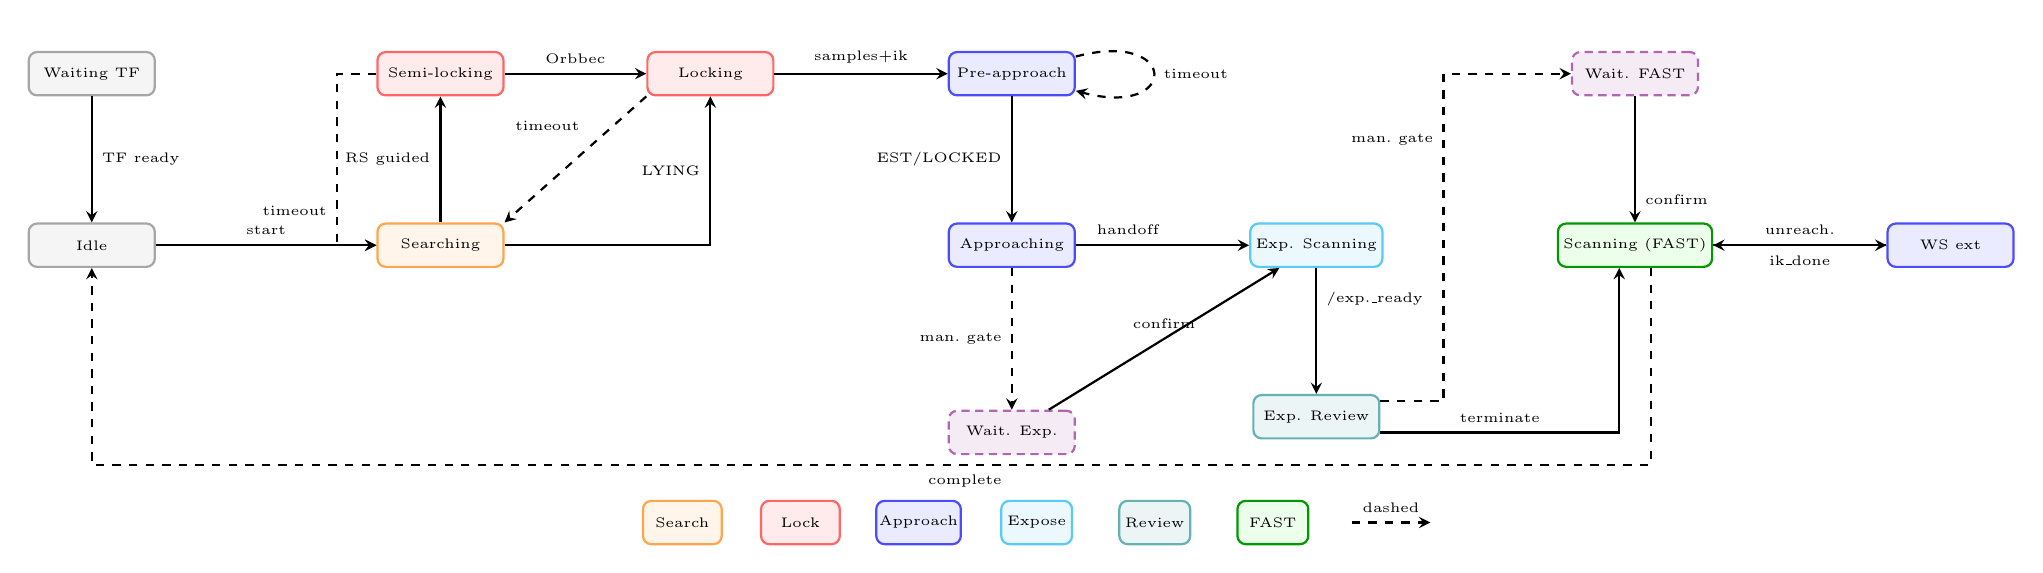
\begin{tikzpicture}[
    node distance = 1.6cm and 1.8cm,
    auto,
    >=stealth,
    state/.style   = {rectangle, rounded corners=3pt, draw, minimum width=1.6cm,
                      minimum height=0.55cm, font=\tiny,
                      fill=white, thick, inner sep=2pt},
    search/.style  = {state, draw=orange!70, fill=orange!8},
    lock/.style    = {state, draw=red!60, fill=red!8},
    approach/.style = {state, draw=blue!70, fill=blue!8},
    expose/.style  = {state, draw=cyan!65, fill=cyan!8},
    review/.style  = {state, draw=teal!60, fill=teal!8},
    scan/.style    = {state, draw=green!60!black, fill=green!8},
    idle/.style    = {state, draw=gray!70, fill=gray!8},
    wait/.style    = {state, draw=violet!60, fill=violet!8, densely dashed},
    trans/.style   = {->, thick, font=\tiny},
    transd/.style  = {->, thick, dashed, font=\tiny},
    every label/.style = {font=\tiny}
  ]

  % ── Column 1: Init (x≈0.0) ──────────────────────────────────
  \node[idle]  (wtf)                                  {Waiting TF};
  \node[idle]  (idl)  [below=of wtf]                   {Idle};

  % ── Column 2: Search / Lock (x≈2.8) ─────────────────────────
  \node[search] (sr)  [right=2.8cm of idl]                    {Searching};
  \node[lock]   (sl)  [above=of sr]                            {Semi-locking};
  \node[lock]   (lk)  [right=of sl]                            {Locking};

  % ── Column 3: Approach + Exposure (x≈6.2) ──────────────────
  \node[approach] (pa) [right=2.2cm of lk]                     {Pre-approach};
  \node[approach] (ap) [below=of pa]                            {Approaching};
  \node[wait]     (we) [below=1.8cm of ap]                        {Wait. Exp.};
  \node[expose]   (es) [right=2.2cm of ap]                      {Exp. Scanning};
  \node[review]   (er) [below=of es]                            {Exp. Review};

  % ── Column 4: FAST (x≈10.2) ─────────────────────────────────
  \node[scan]    (sc) [right=2.2cm of es]                      {Scanning (FAST)};
  \node[wait]    (wf) [above=of sc]                            {Wait. FAST};
  \node[approach] (ws) [right=2.2cm of sc]                     {WS ext};

  % ── Transitions ─────────────────────────────────────────────

  % Init
  \draw[trans] (wtf) -- node[right]{\tiny TF ready} (idl);
  \draw[trans] (idl) -- node[above]{\tiny start} (sr);

  % Search / Lock
  \draw[trans] (sr)  -- node[left]{\tiny RS guided} (sl);
  \draw[trans] (sl)  -- node[above]{\tiny Orbbec} (lk);
  \draw[transd] (sl.west) -- ++(-0.5,0) |- node[pos=0.4,left]{\tiny timeout} (sr.west);
  \draw[trans] (sr)  -| node[above left,pos=0.7]{\tiny LYING} (lk);
  \draw[transd] (lk.south west) -- node[above left,pos=0.4,yshift=2pt]{\tiny timeout} (sr.north east);

  % Lock → Pre-approach
  \draw[trans] (lk)  -- node[above]{\tiny samples+ik} (pa);

  % Pre-approach → Approaching
  \draw[trans] (pa)  -- node[left]{\tiny EST/LOCKED} (ap);
  \draw[transd] (pa) to[loop right] node[right]{\tiny timeout} (pa);

  % Approaching → Exposure (conditional gate)
  \draw[trans] (ap.east) -- node[above,pos=0.3]{\tiny handoff} (es.west);
  \draw[transd] (ap) -- node[left]{\tiny man.\ gate} (we);

  % Waiting Exposure → Exposure Scanning
  \draw[trans] (we) -- node[above]{\tiny confirm} (es);

  % Exposure Scanning → Exposure Review
  \draw[trans] (es) -- node[right,near start]{\tiny /exp.\_ready} (er);

  % Exposure Review → FAST (conditional gate)
  \draw[trans] ([yshift=-0.2cm]er.east) -| node[above,pos=0.25]{\tiny terminate} ([xshift=-0.2cm]sc.south);
  \draw[transd] ([yshift=0.2cm]er.east) -- ++(0.8,0) |- node[left,pos=0.4]{\tiny man.\ gate} (wf.west);

  % Waiting FAST → Scanning
  \draw[trans] (wf.south) -- node[below right,pos=0.7]{\tiny confirm} (sc.north);

  % Scanning ↔ WS ext
  \draw[trans] (sc) -- node[above]{\tiny unreach.} (ws);
  \draw[trans] (ws) -- node[below]{\tiny ik\_done} (sc);

  % Complete → Idle (passes below all states)
  \draw[transd] ([xshift=+0.2cm]sc.south) -- ++(0,-2.5) -|
    node[pos=0.22,below]{\tiny complete} (idl.south);

  % ── Legend ──────────────────────────────────────────────────
  \node[state, draw=orange!70, fill=orange!8, minimum width=1.0cm,
        font=\tiny, inner sep=1pt] at (7.5, -5.7) {Search};
  \node[state, draw=red!60, fill=red!8, minimum width=1.0cm,
        font=\tiny, inner sep=1pt] at (9.0, -5.7) {Lock};
  \node[state, draw=blue!70, fill=blue!8, minimum width=1.0cm,
        font=\tiny, inner sep=1pt] at (10.5, -5.7) {Approach};
  \node[state, draw=cyan!65, fill=cyan!8, minimum width=0.9cm,
        font=\tiny, inner sep=1pt] at (12.0, -5.7) {Expose};
  \node[state, draw=teal!60, fill=teal!8, minimum width=0.9cm,
        font=\tiny, inner sep=1pt] at (13.5, -5.7) {Review};
  \node[state, draw=green!60!black, fill=green!8, minimum width=0.9cm,
        font=\tiny, inner sep=1pt] at (15.0, -5.7) {FAST};
  \draw[transd, thick] (16.0, -5.7) -- node[above,font=\tiny]{dashed} ++(1.0,0);

\end{tikzpicture}
}
  \caption{Mission \ac{FSM} with 13 states. Dashed transitions are
           perception-driven; solid transitions are geometry-driven.}
  \label{fig:fsm}
\end{figure*}

\begin{figure}[t]
  \centering
  \resizebox{\columnwidth}{!}{% ============================================================
%  SYSTEM BLOCK DIAGRAM — 5 columns + injury detection + web UI
% ============================================================
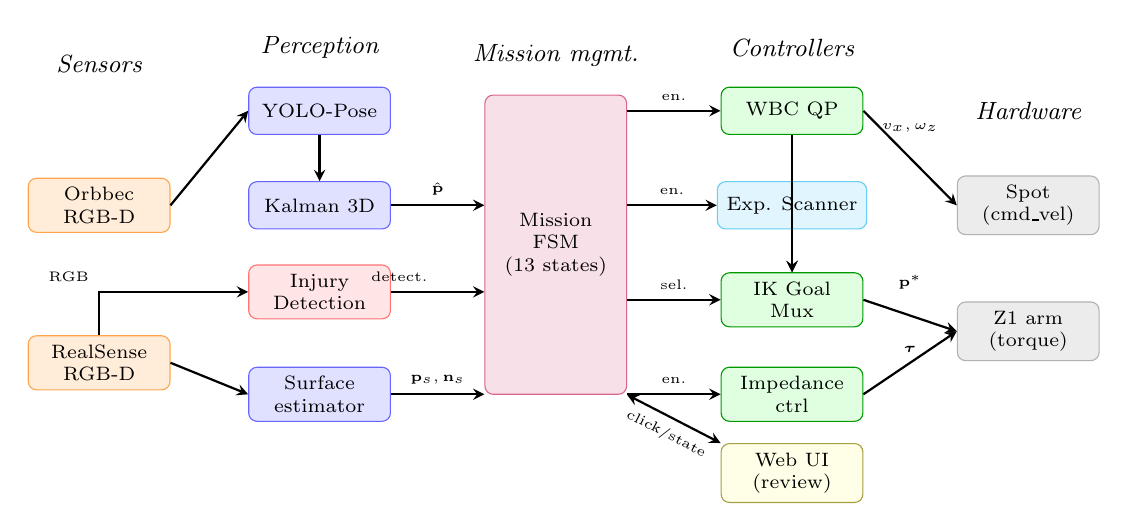
\begin{tikzpicture}[
    >=stealth,
    arr/.style    = {->, thick},
    arrb/.style   = {<->, thick},
    box/.style    = {rectangle, draw, rounded corners=3pt,
                     minimum width=1.8cm, minimum height=0.60cm,
                     font=\scriptsize, align=center, fill=white},
    sensor/.style = {box, fill=orange!15, draw=orange!70},
    percep/.style = {box, fill=blue!12,   draw=blue!60},
    injury/.style = {box, fill=red!10,    draw=red!55},
    fsmbox/.style = {box, fill=purple!12, draw=purple!60,
                     minimum width=1.8cm, minimum height=3.8cm},
    ctrl/.style   = {box, fill=green!12,  draw=green!60!black},
    expctrl/.style = {box, fill=cyan!12,  draw=cyan!60},
    web/.style    = {box, fill=yellow!10, draw=yellow!60!black},
    hw/.style     = {box, fill=gray!15,   draw=gray!60},
    lbl/.style    = {font=\small\itshape},
  ]

  % ── Column x: 0  2.8  5.8  8.8  11.8 ───────────────────────
  % ── Row y:  top rows between +2.6 and -2.4 ────────────────

  % SENSORS
  \node[sensor] (orb)  at ( 0.0,  1.0) {Orbbec\\RGB-D};
  \node[sensor] (rs)   at ( 0.0, -1.0) {RealSense\\RGB-D};

  % PERCEPTION
  \node[percep] (yolo) at ( 2.8,  2.2) {YOLO-Pose};
  \node[percep] (kf)   at ( 2.8,  1.0) {Kalman 3D};
  \node[injury] (inj)  at ( 2.8, -0.1) {Injury\\Detection};
  \node[percep] (surf) at ( 2.8, -1.4) {Surface\\estimator};

  % FSM
  \node[fsmbox] (fsm)  at ( 5.8,  0.5) {Mission\\FSM\\(13 states)};

  % CONTROLLERS
  \node[ctrl]  (wbc)  at ( 8.8,  2.2) {WBC QP};
  \node[expctrl] (exp) at (8.8,  1.0) {Exp. Scanner};
  \node[ctrl]  (mux)  at ( 8.8, -0.2) {IK Goal\\Mux};
  \node[ctrl]  (imp)  at ( 8.8, -1.4) {Impedance\\ctrl};

  % WEB UI
  \node[web] (webui) at ( 8.8, -2.4) {Web UI\\(review)};

  % HARDWARE
  \node[hw] (spot) at (11.8,  1.0) {Spot\\(cmd\_vel)};
  \node[hw] (z1)   at (11.8, -0.6) {Z1 arm\\(torque)};

  % ── Sensors → Perception ────────────────────────────────────
  \draw[arr] (orb.east)  -- (yolo.west);
  \draw[arr] (yolo.south) -- (kf.north);
  \draw[arr] (rs.east)   -- (surf.west);
  \draw[arr] (rs.north)  |- node[above left,font=\tiny]{RGB} (inj.west);

  % ── Perception → FSM ────────────────────────────────────────
  \draw[arr] (kf.east)   -- node[above,font=\tiny]{$\hat{\mathbf{p}}$}
             (fsm.west |- kf);
  \draw[arr] (inj.east)  -- node[above left,font=\tiny]{detect.}
             (fsm.west |- inj);
  \draw[arr] (surf.east) -- node[above,font=\tiny]{$\mathbf{p}_s,\mathbf{n}_s$}
             (fsm.west |- surf);

  % ── FSM → Controllers ───────────────────────────────────────
  \draw[arr] (fsm.east |- wbc) -- node[above,font=\tiny]{en.} (wbc.west);
  \draw[arr] (fsm.east |- exp) -- node[above,font=\tiny]{en.} (exp.west);
  \draw[arr] (fsm.east |- mux) -- node[above,font=\tiny]{sel.}(mux.west);
  \draw[arr] (fsm.east |- imp) -- node[above,font=\tiny]{en.} (imp.west);

  % ── WBC → Mux + Exp Scanner → Mux ──────────────────────────
  \draw[arr] (wbc.south) -- (mux.north);
  \draw[arr] (exp.south) -- (mux.north);

  % ── FSM ↔ Web UI ────────────────────────────────────────────
  \draw[arrb] (fsm.south east) -- node[below,font=\tiny,sloped]{click/state} (webui.north west);

  % ── WBC → Spot ──────────────────────────────────────────────
  \draw[arr] (wbc.east) --
           node[above,font=\tiny,yshift=2mm]{$v_x,\omega_z$} (spot.west);

  % ── Mux → Z1 ────────────────────────────────────────────────
  \draw[arr] (mux.east) --
             node[above,font=\tiny,yshift=2mm]{$\mathbf{p}^*$}
             (z1.west);

  % ── Imp → Z1 ────────────────────────────────────────────────
  \draw[arr] (imp.east) --
             node[above,font=\tiny]{$\boldsymbol{\tau}$}
             (z1.west);

  % ── Column labels ────────────────────────────────────────────
  \node[lbl] at ( 0.0,  2.8) {Sensors};
  \node[lbl] at ( 2.8,  3.0) {Perception};
  \node[lbl] at ( 5.8,  2.9) {Mission mgmt.};
  \node[lbl] at ( 8.8,  3.0) {Controllers};
  \node[lbl] at (11.8,  2.2) {Hardware};

\end{tikzpicture}
}
  \caption{System block diagram. The six-layer architecture spans sensors,
           perception, mission \ac{FSM}, planning, control, and hardware.
           Dashed arrows denote operator-triggered or posture-optimisation
           paths.}
  \label{fig:system_block}
\end{figure}

\subsection{Web-Based Operator Interface}

Full autonomy in emergency assessment is neither feasible nor desirable: the
operator must retain the ability to override or re-inspect regions of clinical
interest. \ac{TERESA} bridges this gap with a web interface that translates a
single 2D click on the Body Map into a 3D whole-body repositioning
command---posture optimisation, base navigation, and arm trajectory
replay---without manual teleoperation.

The \ac{TERESA} web interface provides dual-camera monitoring and robot control
via a browser-based dashboard. During exposure
review, the RealSense overlay renders the scan grid as clickable markers; each
click triggers a full re-positioning sequence---posture optimisation, settle,
and \ac{IK} trajectory replay---within the same \ac{ROS}~2 topic protocol used
for autonomous operation. A manual/automatic scan gate toggle allows the
operator to require explicit confirmation before advancing between mission
phases. All web commands are mirrored on the keyboard controller for
redundancy. Fig.~\ref{fig:web_interface} shows the interface during review.

\begin{figure}[t]
  \centering
  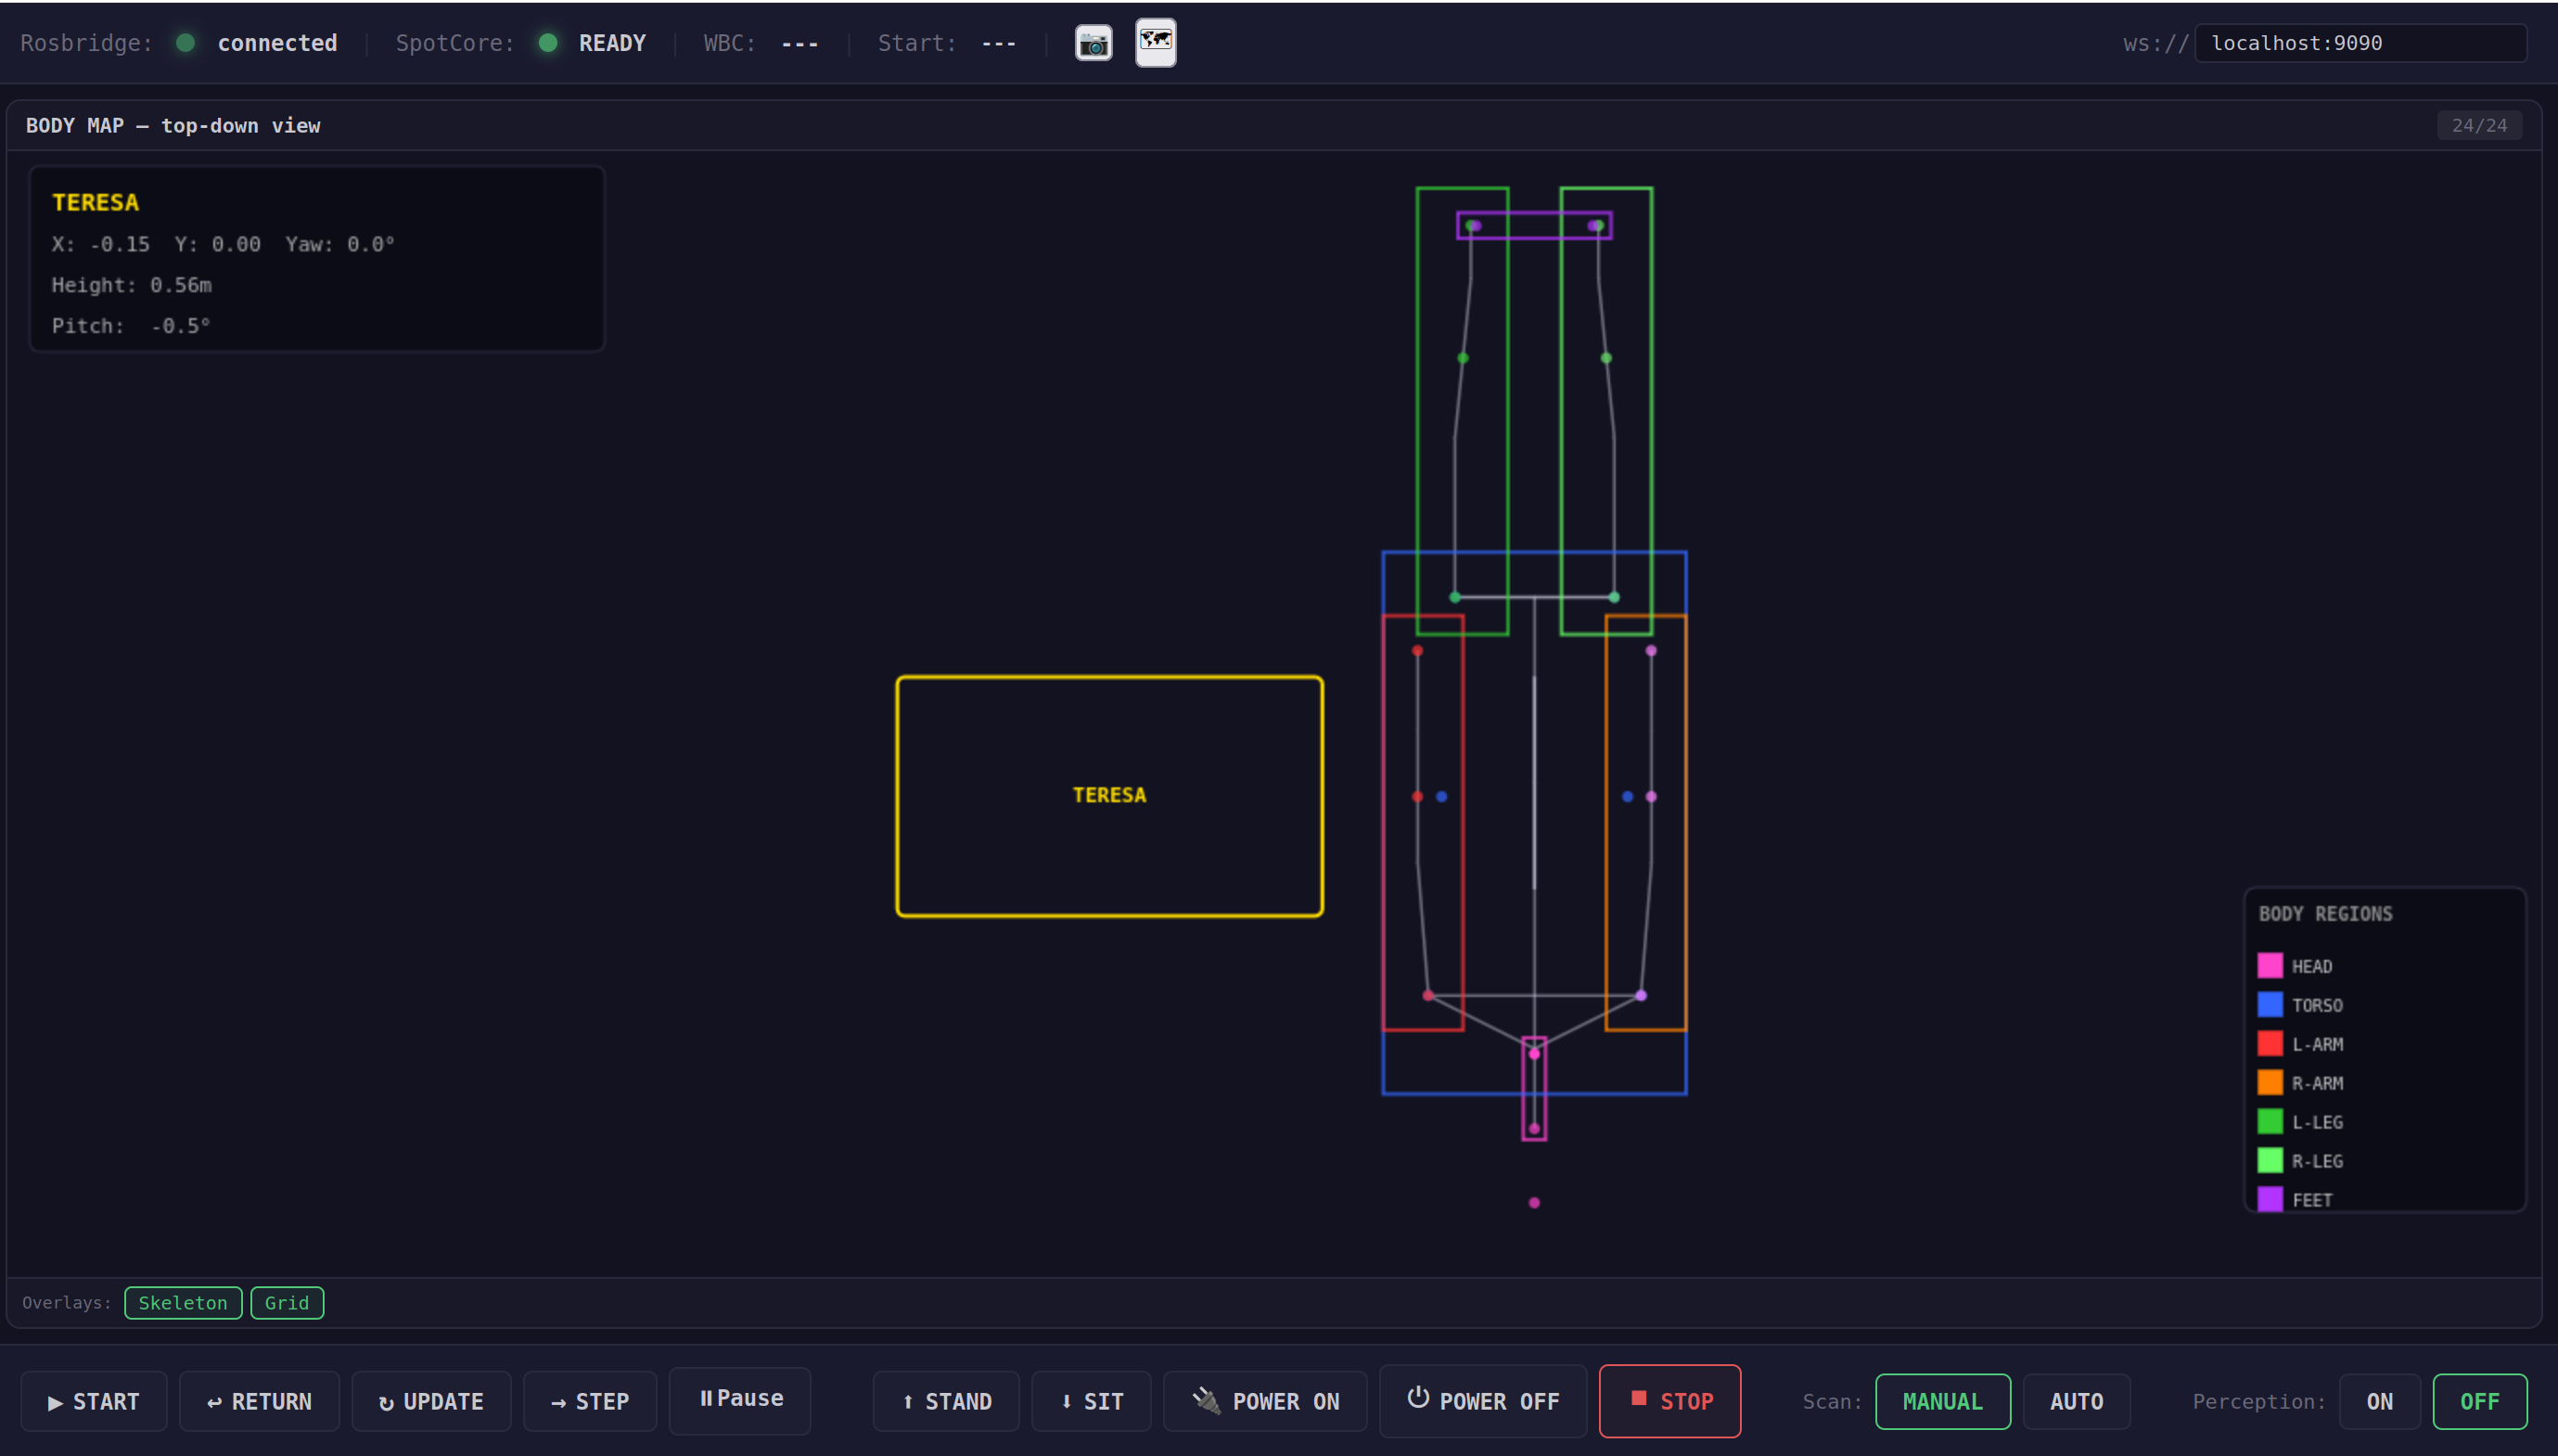
\includegraphics[width=\columnwidth]{figures/Web_interface}
  \caption{Web-based operator interface during the exposure scanning phase. The
           Body Map (top-down view) shows the patient mannequin skeleton with
           colour-coded body regions, the exposure scan grid points, and the Spot
           robot position (yellow). The info panel (top-left) displays Spot's
           current posture parameters. During exposure review, the operator can
           click any grid marker to command the robot to re-inspect that body
           region.}
  \label{fig:web_interface}
\end{figure}

% ============================================================
%  V. EXPERIMENTAL RESULTS
% ============================================================
\section{Experimental Results}
\label{sec:experimental_results}

\subsection{Experimental Setup}

Experiments ran on the physical Spot+Z1 platform with an Orbbec Femto Bolt on
Spot's body and a RealSense D435 at the \ac{EE}, computing across SpotCore
and an external PC over \ac{ROS}~2 Jazzy.  Ten supine patient
positions were defined (\SI{2}{\metre}--\SI{4}{\metre}, $\pm\SI{45}{\degree}$
angular offset); each ran in both modes below, yielding twenty paired trials.

\begin{itemize}
  \item \textbf{Baseline}: sequential stop-and-manipulate. Fixed three-pose scan
        after navigation, no concurrency.
  \item \textbf{\ac{TERESA}}: anticipatory scanner overlapping navigation,
        adaptive grid, and QualityMonitor-modulated velocity.
\end{itemize}

Metrics: total mission time, idle time, scan overlap (fraction of body scan
completed before handoff), \ac{EE} positioning error at each \ac{FAST} point,
and lock time.

\subsection{Search Phase: Whole-Body Coverage and Dual-Sensor Lock}

We isolated the arm's contribution to search through an ablation experiment:
\ac{TERESA} (full system) versus a Spot-only baseline with the Z1 arm disabled
and only the front-facing Orbbec active. Twenty trials were conducted at five
body yaw angles ($0^\circ$--$180^\circ$, two repetitions each), measuring
time to Orbbec posture confidence $\geq$ \num{0.70}.

With the arm's seven scanning poses providing full \SI{360}{\degree} coverage
from a single base position, \ac{TERESA} required no base rotation: frontal
patients were detected near-instantly, the rest during the scan, yielding a
mean of \SI{3.2 \pm 1.1}{\second}. Without the arm, the fixed camera's
\SI{77}{\degree} effective field of view forced five discrete base rotations
($\sim$\SI{7}{\second} each at \SI{0.2}{\radian\per\second}, plus
\SI{2.0}{\second} dwell), giving \SI{14.8 \pm 2.3}{\second}---a
\textbf{5.0}$\times$ slowdown. A \num{10000}-trial Monte Carlo simulation
confirmed this ratio across all patient orientations.

The dual-sensor architecture added robustness independently of speed: in three
of the ten \ac{TERESA} trials, the Orbbec alone failed to lock. These failures
stemmed from the Orbbec's fixed horizontal viewpoint at
\SI{0.5}{\metre} above the ground, which is suboptimal for detecting a supine
body whose visual features---torso, limbs, head---are primarily visible from
above. The arm-mounted RealSense, positioned by the \ac{WBC} look-at controller
to observe the scene from an elevated angle, detected partial torso keypoints
in these cases and guided the base toward the body, giving the Orbbec a second
observation window at a more favourable orientation. Without this redundancy,
these trials would have resumed the coarse search cycle, adding
$\sim$\SI{14}{\second}. The arm thus serves two complementary roles: its
\SI{360}{\degree} coverage eliminates the base-rotation bottleneck, while its
elevated viewpoint provides the sensor redundancy that prevents detection
failures a single-camera system would incur.

\subsection{End-to-End Mission Performance}

Across all twenty end-to-end trials, \ac{TERESA} reduced total mission time
from \SI{100.2 \pm 8.1}{\second} to \SI{89.7 \pm 7.3}{\second} (\SI{10.5}{\percent}).
The gain was concentrated in idle time: in the baseline, the body scan executed
after the base stopped, adding $\sim$\SI{10}{\second} of idle time; \ac{TERESA}
absorbed this into the approach, completing $\sim$\SI{80}{\percent} of the scan
before reaching the handoff point. The adaptive scan grid accelerated this
further: in the majority of trials, torso keypoints were already resolved before
approach, and the grid automatically selected the minimal two-pose pattern
rather than the full three-pose sweep. Pre-planned body reconfiguration reduced
probe positioning error from \SI{44.7 \pm 5.2}{\milli\metre} to
\SI{29.8 \pm 4.1}{\milli\metre}, with the largest improvement at lateral
\ac{FAST} targets. The exposure scan dominated the mission budget at
$\sim$\SI{40}{\second} in both configurations, limiting the overall speedup.
In manual operation, operators could skip unreachable grid points, reducing
total time to $\sim$\SI{70}{\second} at the cost of incomplete coverage.

\subsection{Whole-Body Reconfiguration}

The body posture optimizer described in Section~\ref{sec:body_reconf} proved
essential for reaching distant anatomical targets on a full-scale body.  We
compared four configurations of increasing capability.  The fixed nominal
posture (height \SI{0}{\metre}, pitch \SI{0}{\degree}, no base displacement),
representing Spot's default standing pose, reached only
$\sim$\SI{40}{\percent} of exposure grid points and $\sim$\SI{50}{\percent}
of \ac{FAST} targets.  A heuristic posture---moderately lowered
($\sim$\SI{-0.15}{\metre}) with a slight forward pitch
($\sim$\SI{5}{\degree})---improved these to $\sim$\SI{55}{\percent} and
$\sim$\SI{65}{\percent}, but could not adapt to individual point locations.
The 2D optimiser, selecting the best $(h, \varphi)$ per point via grid search
with \ac{IK}-driven retry, raised completion to $\sim$\SI{70}{\percent}
(exposure) and $\sim$\SI{85}{\percent} (\ac{FAST}).  Finally, the 3D
optimiser added longitudinal base walking $dy$ with the regularised cost
$J = \|\mathbf{p} - \mathbf{p}_{\mathrm{sweet}}\| + \lambda\,|dy|$
($\lambda = 0.50$), achieving $\sim$\SI{85}{\percent} and
\SI{100}{\percent} respectively.  The penalty encouraged height and pitch
adjustments over walking---reducing energy consumption and producing smoother
motion---while still allowing displacement when necessary.  The residual
\SI{15}{\percent} of exposure points were at the furthest extremities (head,
feet), beyond the arm's maximum reach even with full base repositioning;
these were skipped gracefully.  Each tier contributed measurably to mission
completeness, with the movement penalty ensuring that base walking is used
only when strictly needed.

\subsection{Exposure Body Scanning and Injury Detection}

The exposure pipeline was evaluated with XX trials on supine patients,
generating XX~$\pm$~XX scan points. Per-point dwell of
\SI{2}{\second} yielded scan durations of XX~$\pm$~XX\,s. The injury detection pipeline achieved a wound
recall of XX\,\% and burn classification accuracy of XX\,\%,
with a false positive rate of XX per scan on average. The 3D localisation error
of detected injuries was XX~$\pm$~XX\,mm.

\subsection{Discussion}

The results demonstrate that treating body posture as an active perceptual
resource yields measurable improvements in both mission speed and
completeness.  The arm's \SI{360}{\degree} coverage eliminates the
base-rotation bottleneck during search, while body reconfiguration lifts
completion from $\sim$\SI{40}{\percent} to near-\SI{100}{\percent}.  The
dual-sensor architecture prevents detection failures that a single-camera
system would incur.  Several limitations remain: the system assumes a
single stationary patient on flat terrain; ultrasound image quality and
clinical scanning pressure were not evaluated; and the injury detection
pipeline relies on pre-trained models whose performance may vary across
wound types and skin tones.  These aspects are the subject of ongoing work.

% ============================================================
%  VI. CONCLUSION
% ============================================================
\section{Conclusion}
\label{sec:conclusion}

This paper presented \ac{TERESA}, a legged mobile manipulator for autonomous
emergency assessment. The core contribution is a whole-body active perception
framework that treats body posture---height, pitch, and yaw---as a perceptual
resource, closing the perception-action loop at the whole-body level.
Experiments on the physical Spot+Z1 platform demonstrated that the arm's
\SI{360}{\degree} coverage accelerates search by a factor of five over a
fixed-camera baseline, the dual-sensor lock prevents single-camera detection
failures, anticipatory scanning eliminates idle time by completing the body
scan concurrently with approach, and body reconfiguration lifts anatomical
target completion from \SI{40}{\percent} to \SI{100}{\percent} for \ac{FAST}
targets.  The exposure pipeline integrates zero-shot wound detection with an
interactive web-based review interface.

Several limitations remain: the system assumes a single stationary mannequin on
flat terrain; ultrasound image quality and clinical scanning pressure were not
evaluated; and injury detection relies on pre-trained models whose performance
may vary across wound types and skin tones.  Future work will extend
\ac{TERESA} to multi-patient scenarios, clinical ultrasound acquisition with
impedance-controlled probe contact, and ultimately the full \ac{ABCDE}
protocol, providing a complete autonomous primary survey for emergency triage.


% ── Bibliography ────────────────────────────────────────────
\bibliographystyle{IEEEtran}
\bibliography{references}

\end{document}
